\newpage

\section{Circuit Playground (CPX/CPB) Modules}

\subsection{Parts List}

\begin{enumerate}[itemsep=-5pt]
\item Laptop
\item CPX/CPB
\item USB Cable
\end{enumerate}

\subsection{Learning Objectives}
\begin{enumerate}[itemsep=-5pt]
\item Understand the different sensors on the Circuitplayground
\item Learn the difference between high level and low level control
\item Get more practice plotting data from onboard sensors
\end{enumerate}

\subsection{Extra Help}
If you need extra help on this assignment I have uploaded a youtube video where I \href{https://www.youtube.com/watch?v=ceI0uw3ICE0}{read the temperature and accelerometer from the CircuitPlayground Bluefruit}

\subsection{Getting Started}

The CPX has numerous built-in sensors. These include a light sensor, an IR sensor, an accelerometer, a microphone, a speaker, some neopixels, a temperature sensor and 8 analog inputs with ADCs and even I2C (pronounced I squared C - it’s a kind of serial communication) that you can use to easily hook up more sensors to it. We’re not going to utilize all of these sensors since that would be a rather large project. Instead we’re going to learn how to use the temperature, light and sound sensors as well as the accelerometer. For each of these examples there is a relatively easy way to access the sensors using a built-in module called {\it adafruit\_circuitplayground.express} if you are using the CPX. If you are using the CPB you need to type {\it adafruit\_circuitplayground.bluefruit}. It’s a very nice module because it imports everything on the board. The problem is you can run into module conflicts. This happens when two different modules try to access the same pins on the CP. Sometimes if you import {\it adafruit\_circuitplayground} you won’t be able to import some other modules. {\bf Note you might need to add the {\it adafruit\_circuitplayground} library to your lib/ folder on your CIRCUITPY drive}. Due to this module conflict issue, there are some low level control commands you can use to access each of the sensors on board. We’re obviously going to learn the low level control method first and then I’ll show you how to access the sensors using the {\it adafruit\_circuitplayground} module. {\bf If you get a “currently in use” error it means you have a module conflict. Hence why I’m showing you the low level control method}.

\subsection{Low Level Control}

\subsubsection{Light}

The light sensor on the CPX is just a simple photocell wired in series with a resistor. There is a lab on photocells (See chapter \ref{s:photocell} if you'd like to do that lab first to learn about photocells. The GND leg of the photocell is connected to pin A8. You can check the pin by looking at the graphic of an eye on the CPX and taking a look at the digital pin next to it. We’ve already learned how to {access analog pins (See chapter \ref{s:voltage}) in a previous lab so just use the \href{https://github.com/cmontalvo251/Microcontrollers/blob/master/Circuit_Playground/CircuitPython/Analog/analog_simple.py}{code from that lab} and change the pin to A8. Here’s what my code looks like when I change the pin to A8. I also brought the Plotter up and moved my finger in front of the light to make sure the light was working. Verify that your CPX responds the same way before moving on.
\begin{figure}[H]
  \begin{center}
    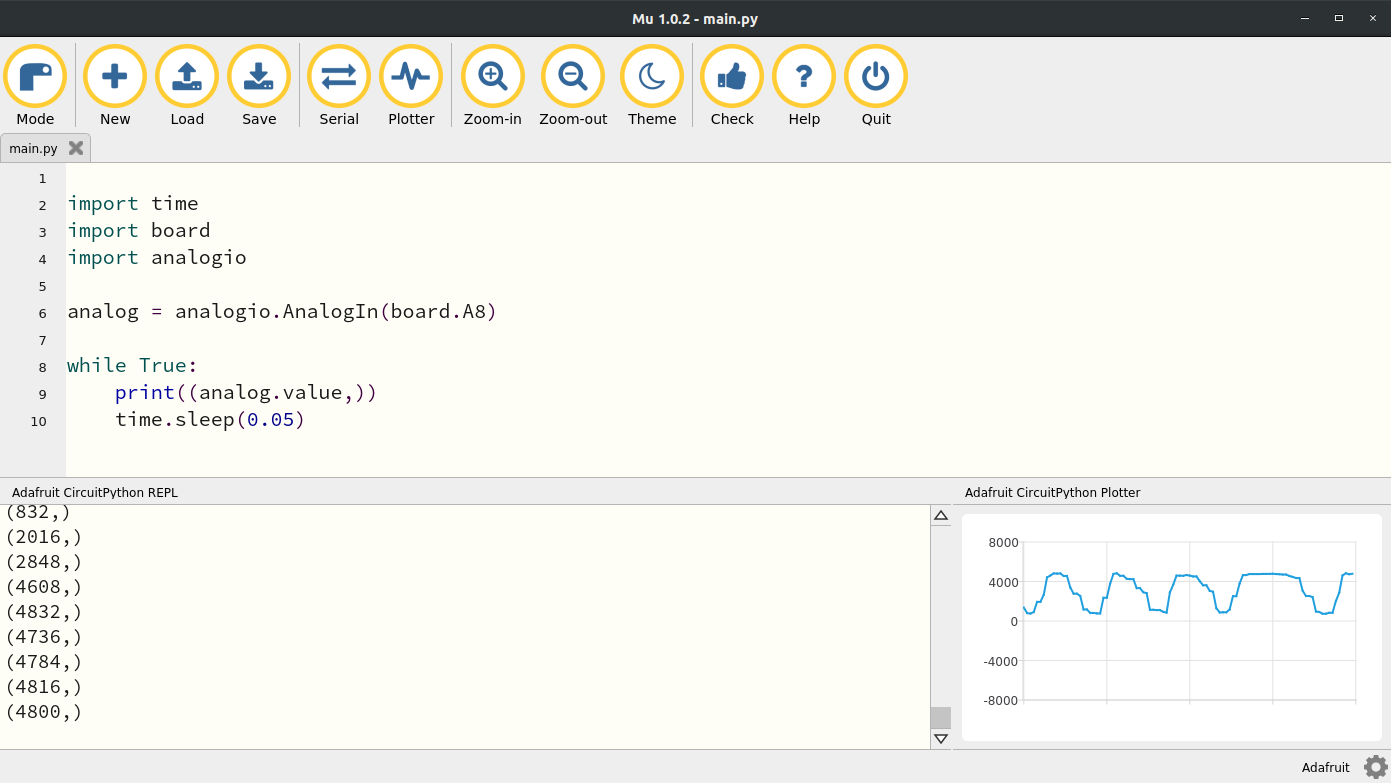
\includegraphics[width=\textwidth]{Figures/modules_light_mu.png}
  \end{center}
\end{figure}
\subsubsection{Sound}
The sound sensor uses the audiobusio library and creates a mic object using the (Pulse Density Modulation) PDM library. You have to set the sample rate and the number of bits to use to capture the data. We’re going to set the bits to 16 to utilize the whole spectrum and then set the sample rate to 16 kHz. It’s not quite 44.1 kHz like most modern microphones but it will do. After creating the mic object we have to compute some root mean squared values and thus two functions are defined before the while true loop in the code. The code itself is shown below. The code starts on line 22 because the first \href{https://learn.adafruit.com/adafruit-pdm-microphone-breakout/circuitpython}{22 lines are copyright from Dan Halbert, Kattni Rembor, and Tony DiCola from Adafruit Industries}. I have edited the code a bit to fit my needs and uploaded \href{https://github.com/cmontalvo251/Microcontrollers/blob/master/Circuit_Playground/CircuitPython/Audio/record_sound_simple.py}{my version to Github}. In the code line 23-27 import standard modules as well as some new ones. The array module is used to create array like matrices. The math module is used to compute functions like cos, sin, and sqrt. Then of course the audiobusio module is used to create the mic object on line 42. Notice the two functions defined on 33 and 39 which create a function for computing the mean and for computing the normalized root mean square value of the data stream. Basically what’s going to happen is we’re going to record 160 samples as defined on line 160. So on line 43 we create a hexadecimal array (hexademical: base 16 hence the num\_bits set to 16 on line 31) with 160 zeros. In the while true loop we’re going to sleep for 0.01 seconds and then record some samples. Since we’re sampling at 16 kHz the time it takes to record 160 samples is 160/16000 = 16/1600 = 1/100 = 0.01 seconds. Since we’re taking 160 samples we need to compute some sort of average which is why the normalized root mean square value is computed on line 48.
\begin{figure}[H]
  \begin{center}
    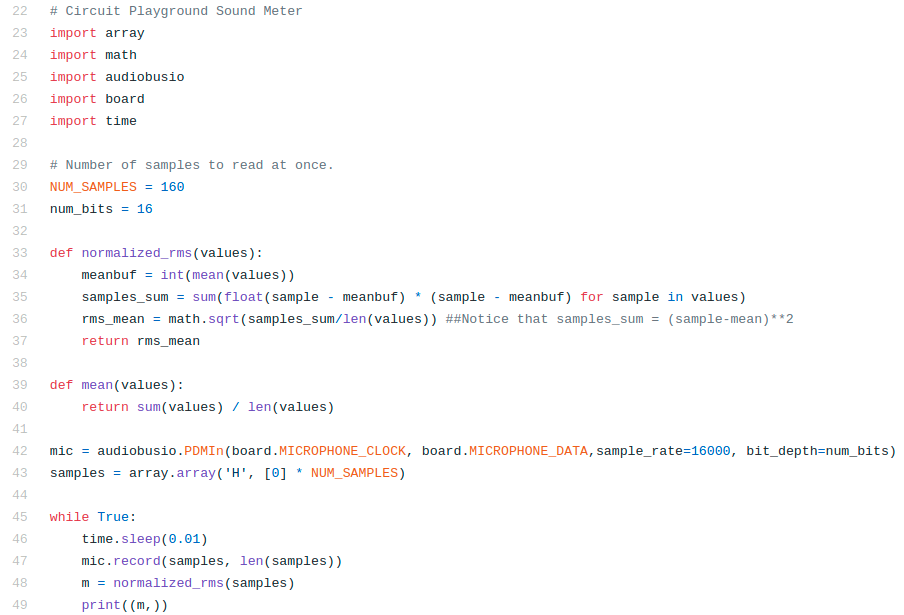
\includegraphics[width=\textwidth]{Figures/sound_code.png}
  \end{center}
\end{figure}
When I run this code and talk normally into the microphone. I get this output in the Plotter. You’ll notice that the data is pretty noisy in the beginning. It’s possible we could increase the number of samples we take each loop by editing line 30 but that would slow down our code. So there’s a tradeoff between filtering here and speed. That’s something will investigate in some later labs.
\begin{figure}[H]
  \begin{center}
    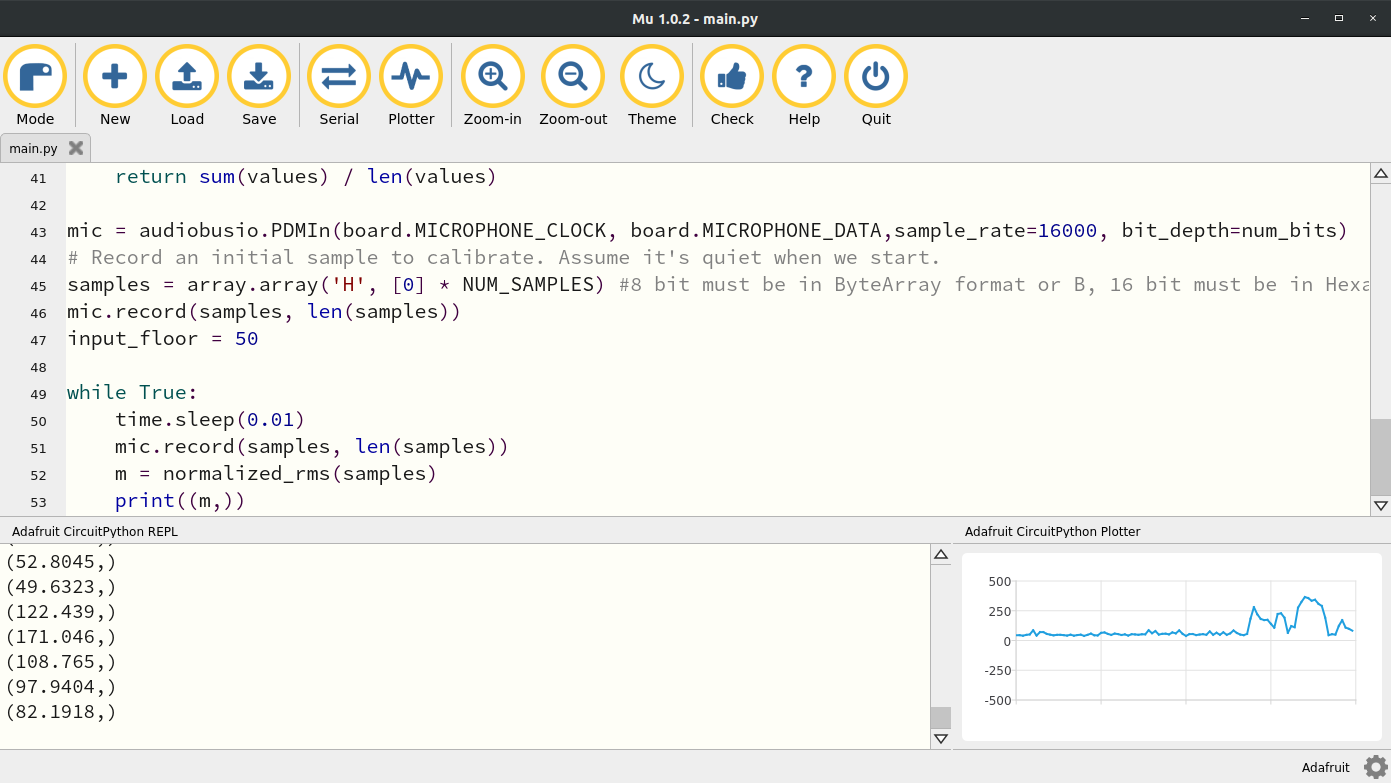
\includegraphics[width=\textwidth]{Figures/sound_mu.png}
  \end{center}
\end{figure}
\subsubsection{Temperature}
The temperature sensor is actually a \href{https://en.wikipedia.org/wiki/Thermistor}{thermistor}. A thermistor is basically a thermometer resistor which means the resistance depends on temperature. This means that you can read the analog signal coming from the thermistor just by reading the analog signal from pin A9. If you look for the thermometer symbol on the CPX you’ll see pin A9. Therefore, it is possible to just use the analogio library and just read in the analog voltage but in order to convert to celsius and then fahrenheit you need to use some heat transfer equations to convert the analog signal to celsius. Thankfully the folks at Adafruit have done it again with an {\it adafruit\_thermistor} module. If you head over to their \href{https://github.com/adafruit/Adafruit_CircuitPython_Thermistor/blob/master/adafruit_thermistor.py}{github on this module} you’ll see the relevant conversion under the definition temperature which at the time of this writing is on line 86. \href{https://learn.adafruit.com/thermistor/circuitpython}{The Adafruit Learn system also does a bit of work to explain the conversion from voltage to temperature}. For now though we will just appreciate the simplicity of the code below which is also \href{https://github.com/cmontalvo251/Microcontrollers/blob/master/Circuit_Playground/CircuitPython/Temp/record_temperature_thermistor.py}{on my Github}.
\begin{figure}[H]
  \begin{center}
    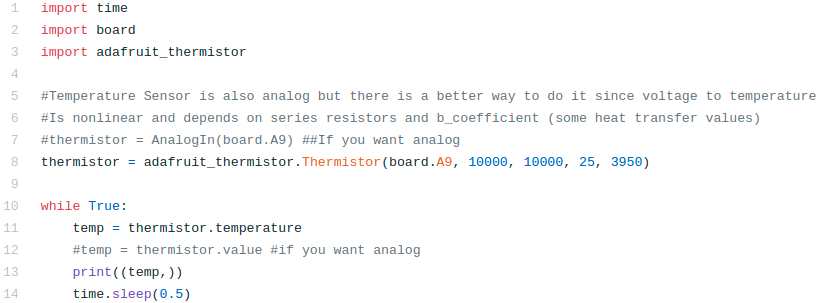
\includegraphics[width=\textwidth]{Figures/thermistor_code.png}
  \end{center}
\end{figure}
As always lines 1-3 import the relevant modules and then line 8 create the thermistor object. You’ll notice the input arguments are the pin which is A9 as well as the resistor values which are in series with the thermistor. These resistors are soldered to the PCB so they are fixed at 10 kOhms. The 25 is for the nominal resistance temperature in celsius of the thermistor and 3950 is the b coefficient which is a heat transfer property. Running this code and then placing my finger on the A9 symbol causes the temperature to rise just a bit. You’ll notice the temperature rise quite quickly when I place my finger on the sensor but when I remove the sensor it takes some time before the sensor cools off. This has to do with the dynamic response of the sensor. We’ll discuss this in some future labs on dynamic measurements. For now you can move on to the accelerometer.
\begin{figure}[H]
  \begin{center}
    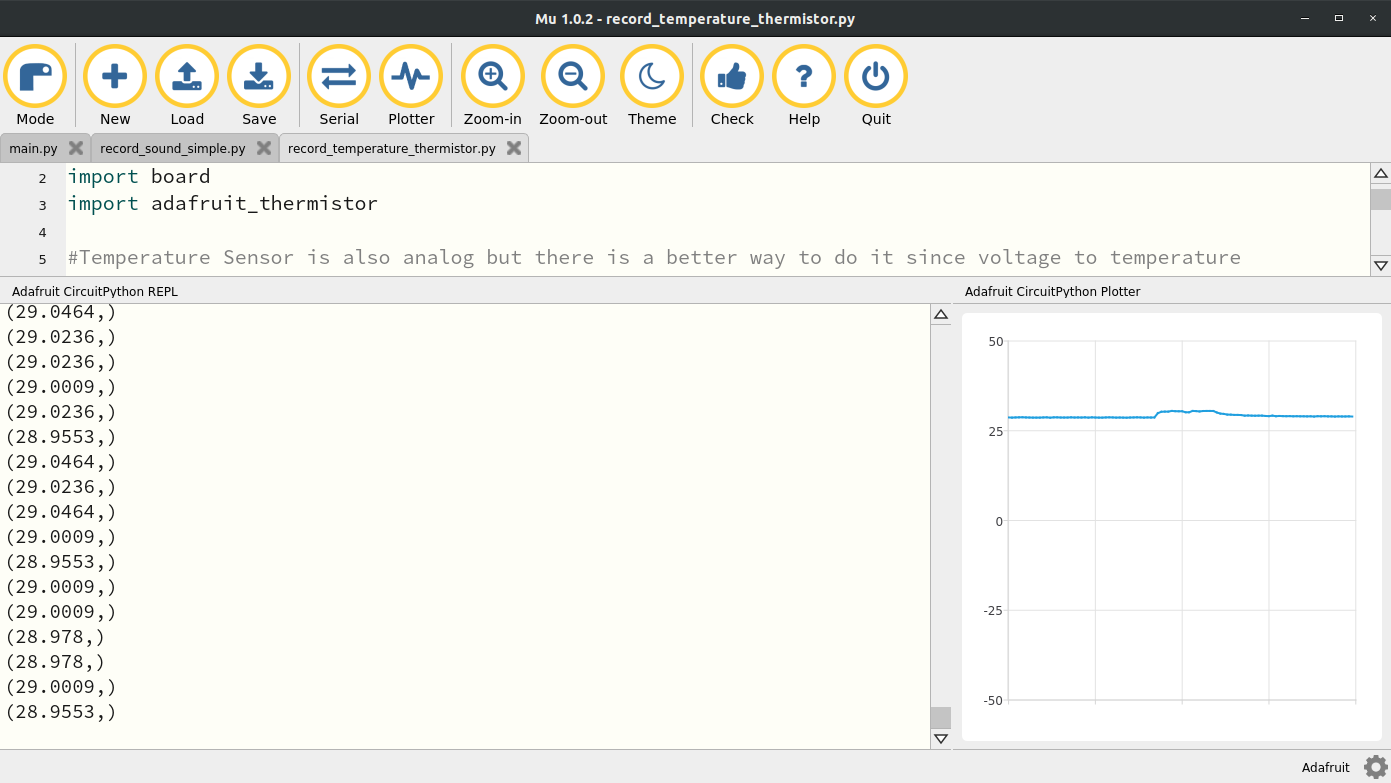
\includegraphics[width=\textwidth]{Figures/thermistor_mu.png}
  \end{center}
\end{figure}
\subsubsection{Accelerometer}
\label{s:modules}
The accelerometer is a 3-axis sensor. As such it is going to spit out not just 1 value but 3 values. Accelerations in x,y and z or North, East, Down or Forward, Side to Side, Up and Down. Since it’s reading 3 values we can’t just read 3 analog signals (we can but the accelerometer chip design didn’t want to do that) so instead we’re going to use the I2C (I like indigo and square C. So I squared C. Not 12C or one two C. It’s I squared C) functionality. I2C is a type of serial communication that allows computers to send strings rather than numbers. It’s a much more complex form of communication but since it’s standard we can just use the busio module which contains the I2C protocol.
\begin{figure}[H]
  \begin{center}
    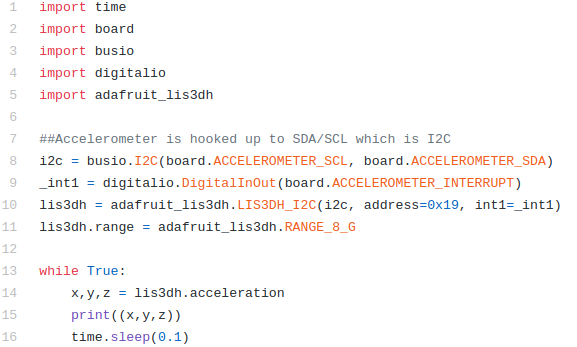
\includegraphics[width=\textwidth]{Figures/accelerometer_code.png}
  \end{center}
\end{figure}
In this code we see alot more imports than normal. In addition to the standard time, board and digitalio modules we need the busio module and the {\it adafruit\_lis3dh}. You might think that LIS3DH is a very weird name for an accelerometer but it’s actually the name of the chip on your CPX. The chip itself is very standard and is well documented on multiple websites. \href{https://www.st.com/en/mems-and-sensors/lis3dh.html}{Here’s one from ST}. You can also buy the \href{https://www.adafruit.com/product/2809?gclid=EAIaIQobChMI98qfjrC86gIVEI_ICh2JtQ-JEAAYAiAAEgJ2_fD_BwE}{chip on a breakout board from Adafruit} and then of course the Adafruit Learn site has plenty of tutorials on \href{https://learn.adafruit.com/circuitpython-hardware-lis3dh-accelerometer/software}{reading Accelerometer data in CircuitPython}. As always I’ve learned what I can from the relevant tutorials and created \href{https://github.com/cmontalvo251/Microcontrollers/blob/master/Circuit_Playground/CircuitPython/Accelerometer/low_level_accel.py}{my own simple version to read the accelerometer data and posted it to Github}. I digress, lines 8-11 of the code do alot. It first uses the SCL and SDA pins to set up an I2C object which establishes serial communication to the accelerometer. Line 9 creates an interrupt which is beyond the scope of this course. Finally, line 10 creates the actual accelerometer object by sending it the I2C pins, the hexadecimal address in the I2C protocol and finally the interrupt pin. Line 11 then sets the range. Line 14 in the while loop is where the x,y and z values of the accelerometer are read and then promptly printed to Serial on line 15. If I run this code and shake the sensor a bit I can get all the values to vary. If you put the CPX on a flat surface, the Z axis will measure something close to 9.81. The units of the accelerometer are clearly in $m/s^2$.
\begin{figure}[H]
  \begin{center}
    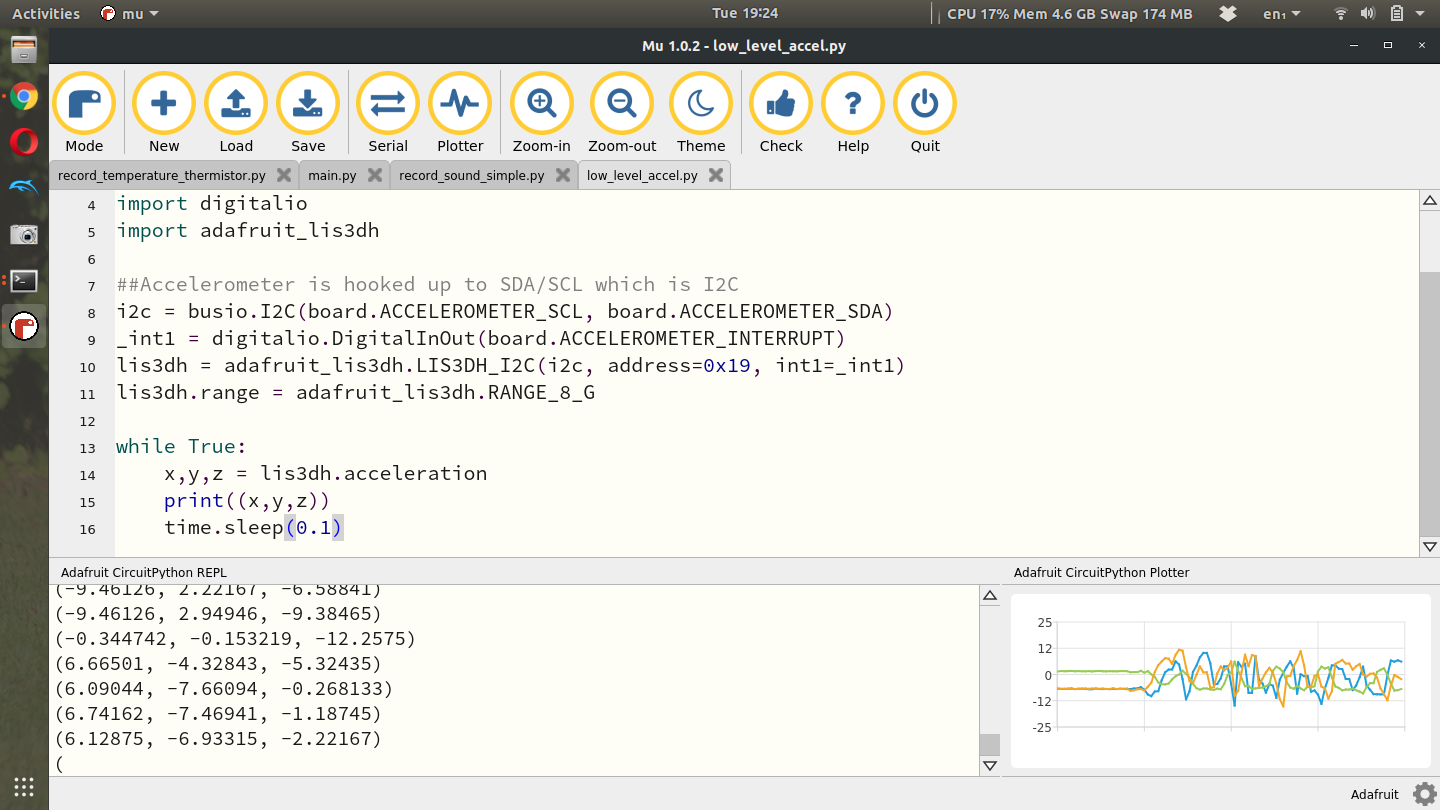
\includegraphics[width=\textwidth]{Figures/accelerometer_mu.png}
  \end{center}
\end{figure}

\subsection{High Level Control}

Alright so we’ve learned the hard way for all the sensors using low level control of the various sensors. Let’s now import the simple adafruit\_circuitplayground.express module. \href{https://learn.adafruit.com/circuitpython-made-easy-on-circuit-playground-express/circuit-playground-express-library}{The Adafruit Learn site offers pretty much every example code snippet you’d ever need for all the different push buttons and sensors on the CPX}. Head over there if you ever need something outside of the scope of this text. As I said before, the main module you need to import is done by adding the following to the top of your code
\begin{verbatim}
from adafruit_circuitplayground.express import cpx
\end{verbatim}
{\bf Note that you need to change that line to adafruit\_circuitplayground.bluefruit import cpb. Then everywhere you see cpx you replace with cpb.}
This will import the cpx module into your working code. From here the commands to read different things are relatively simple. Here are the commands for all the various sensors
\begin{verbatim}
light = cpx.light

x,y,z = cpx.acceleration

temperature = cpx.temperature
\end{verbatim}

There unfortunately is no simple module for the sound sensor. You’ll still need to use the low level control no matter what. According to Adafruit though, if you get the Circuit Playground Bluefruit there is a \href{https://learn.adafruit.com/circuitpython-made-easy-on-circuit-playground-express/sound}{simple way to read the sound level}. Implementing the various sensors into a while loop on my CPX looks like this.
\begin{figure}[H]
  \begin{center}
    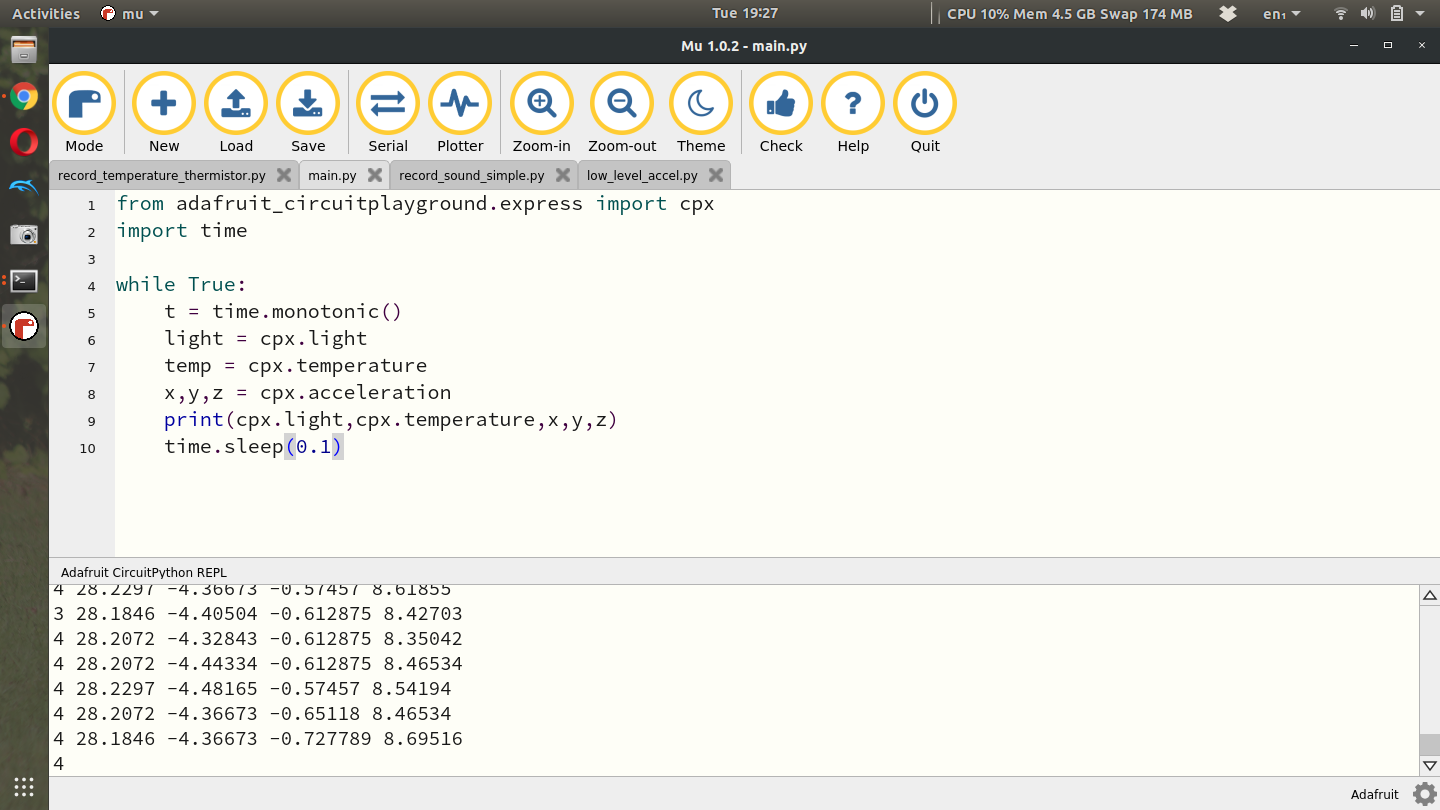
\includegraphics[width=\textwidth]{Figures/high_level_mu.png}
  \end{center}
\end{figure}
I left out the sound sensor stuff just because it kind of messes with the simplicity of the code above. The adafruit\_circuitplayground.express module outputs just as before except for the light sensor. In the low level control we simply computed the voltage across the photocell but the adafruit\_circuitplayground.express module outputs data in \href{https://en.wikipedia.org/wiki/Lux}{Lux}.

\subsection{Assignment}

Using either {\bf low or high level control} take at least 60 seconds of data for each of the sensors above. Make sure log time and the raw sensor value at 1Hz or faster. To make the project more challenging, try and log all sensor data all at once. Import the data onto your desktop and make 4 plots total with time on the x-axis and the sensor data on the y-axis.

Once you've done that upload a PDF with all of the photos and text below included. My recommendation is for you to create a Word document and insert all the photos and text into the document. Then export the Word document to a PDF. For videos I suggest uploading the videos to Google Drive, turn on link sharing and include a link in your PDF.

\begin{enumerate}[itemsep=-5pt]
\item Using the Plotter in Mu, take a video of you plotting light, sound, temperature and acceleration one at a time while varying light, sound, temperature and acceleration individually and watching the plot change in Mu (be sure to be in the video and introduce yourself) - 30\%
\item Copy and paste your CPX code that you used to log data for each of the sensors - 20\%
\item Copy and paste your Python desktop code that you used to plot data for each of the 4 sensors - 20\%
\item Include 4 plots with time on the x-axis and sensor data on the y-axis (No screenshots) - 30\%
\end{enumerate}